\chapter{Hardware vs Software}

In the preceding weeks we've learned about hardware, the physical components that make up computing
systems. Hardware is only half of what constitute computing systems. Software is the ``brain'' of
a computer system that dictates how the hardware should execute. Hardware without software is like
a car without a driver --- it is unable to do much. Similarly, software without hardware to run on
is like a driver without a car, it has nothing to drive. Together software and hardware are able to
perform work in a meaningful and controlled way.

In this section, we will discuss the distinction between hardware and software and how they
interact. As seen in Figure~\ref{fig:hw_sw:layers}, many layers of software sit between the hardware of
our computer systems and the software we use and develop. These layers build up from the hardware and
abstract away many of the complexities of lower levels to provide more and more functionality.

\begin{figure}
\centering
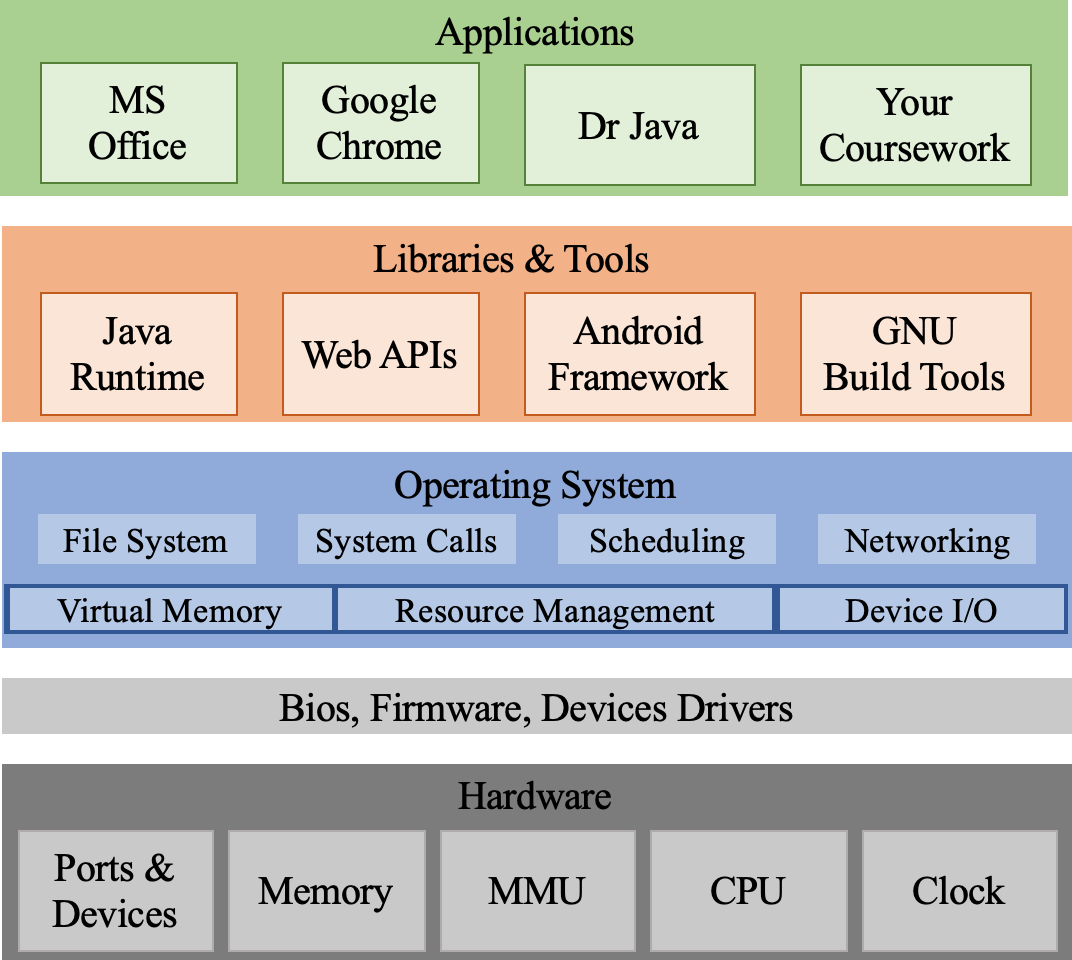
\includegraphics[width=6.5cm]{images/software_layers.png}
\caption{Layers of software built up from hardware. Each providing more abstractions and functionality for higher levels to use.}
\label{fig:hw_sw:layers}
\end{figure}

\section{Hardware}
As discussed previously, hardware is the collection of physical devices that make up a computer.
The hardware performs the actual computations by manipulating electrical currents. Today most
computers are digital, meaning that the computer works by representing data with electrical currents
at a High or Low voltage. We think of these high-voltages at representing on or 1 and low-voltages
as off or 0. The only thing the hardware understands are these voltages. However, there is a direct
translation from these voltages to binary numbers. This representation as binary numbers is often
called the computer's machine language. Not all computers recognize the same machine code language ---
the same sequence of 1's and 0's may not represent the same information on two computers ---
and is often manufacturer dependent.

Often times, manufacturers of computers (more specifically manufacturers of central processing units)
describe what machine language a computer understands by providing another language called
an assymbly language. This assymbly language has a one-to-one translation to machine code language.
This assymbly language is designed to be more human-readable than machine code. (e.g. store x0 M(x1)1000
as opposed to 01100100000000011000, where both mean store the value of register x0 into the memory location
offset by 1000 from the location pointed at by register x1). While each computer manufacturer may
have thier own machinge code for each computer they design, there are far fewer assymbly languages.
Today, the most popular assymbly languages include MIPS, ARM, RISC-V, and Intel x64. With assymbly
languages, computer manufacturers only need to supply the translation from assymbly language
to thier machine code (and thus into high and low voltages).

\section{BIOS and Firmware}
Today, it is very likely that the first software loaded onto any computing device is a firmware.
Firmware is software that helps facilitate other software interacting with the computer device.
One notable firmware, is called the BIOS (Basic Input/Output System). You would be hard-pressed
to find any personal computer or smartphone that doesn't have a BIOS already pre-installed by
the devices manufacturer. A BIOS helps facilitate initial loading of programs onto a computer.
A BIOS will tell the computer to look for a connected device trying to communicate with the
computer (e.g. CD or USB drives). Specifically, a BIOS is the program that helps with installing
and loading an operating system onto a computer.

\section{Operating Systems}
Today it is very hard to find any personal device that doesn't come pre-installed with an
operating system, and if it does the first thing you'll do is install an operating system
onto it. Today the most popular operating systems include MacOS, Windows, Linux, or
various flavors of each. The operating system handles all of the low-level details of the
computer, manages computing resources, and exposes a high-level interface that user-programs
may use. In this sense, the operating system of a computer is like the subconcious parts
of our brain. Things like file-systems, memory-management, processes, threads, scheduling,
user-programs, kernel-programs, and system calls are all designed and implemented by the
operating system. When a user decides to run a program, the operating system will start
the program and hand over control to the program for some time.

At a high-level the operating system is in charge of how to properly run all the
programs the user wants to run. The operating system will handle how to manage
shared resources (memory, cpu-time, IO-devices). These resources are often
requested by the user-program to the operating system through the use of system calls.
These system calls switch control from the user-program to the operating system,
so that the operating system can execute on the programs behalf and help
distribute the shared resources accordingly.

\section{Libraries and Tools}
There are many repeated designs and tricky-to-get-right code that programmers
want to use. Instead of every programmer and program including thier own
version of these repeated designs and code. These are provided to the
end programmer in the forms of tools and libraries. A library is
similar to the system calls provided by the operating system. A library
provides an interface that the programmer can use to have the library
execute code on the programs behalf. Libraries offer a plethora of
functionality includind thread-safe data structures, networking
API's, generating graphics, and many more. Tools are very similar
but instead are there own program that one can interact with
rather than use it as a programming interface. Tools range
from the simple (list contents of folder and simple text-editor)
to the complex (Optimization Solvers, build systems, and IDE'S (Dr. Java)).

\section{Applications}
On top of all of these, sits user programs. These are the programs that
an end user will run, and that you, yourself may write. These build upon
all of the functionality provided by the operating systems, tools,
and libraries to build new and novel applications. There are a limitless
number of applications that you can achieve by using the right
abstractions. Today, popular applications include mobile games,
browsers, word-editors, messenging apps, and much more.

